\documentclass{beamer}
\usepackage{etex}

%\useoutertheme[glossy]{wuerzburg}
\useinnertheme[shadow,outline]{chamfered}
%\usecolortheme{shark}
\usecolortheme{beaver}
\beamertemplatenavigationsymbolsempty

\usefonttheme{professionalfonts}
\let\digamma\relax
\usepackage[scale=0.85,stdmathitalics=true,romanfamily=casual]{lucimatx}
\usefonttheme[stillsansseriftext]{serif}



\usepackage{fancyvrb}

%% Fancy syntax coloring via pygments
\usepackage{minted}
\definecolor{bg}{rgb}{0.95,0.95,0.95}
\usemintedstyle{borland}


\newenvironment{Rcode}
{\VerbatimEnvironment
 \begin{minted}[fontsize=\scriptsize,baselinestretch=1]{r}}%
{\end{minted}}

\newenvironment{Pcode}
{\VerbatimEnvironment
 \begin{minted}[fontsize=\scriptsize,baselinestretch=1]{python}}%
{\end{minted}}

\newenvironment{Code}[1]
{\VerbatimEnvironment
 \begin{minted}[fontsize=\scriptsize,baselinestretch=1]{#1}}%
{\end{minted}}


\usepackage{textfit} % commands \scaletoheight{height}{text} and \scaletowidth{width}{text}

\usepackage{tikz}

\usepackage{tcolorbox}

\newtheorem{Alert}{Alert}
\newtheorem{Highlight}{Highlight}

\newcommand{\Species}[1]{{\rmfamily \itshape #1}}
\newcommand{\Real}{\ensuremath{\mathbb{R}}}
\newcommand{\RealN}{\ensuremath{\mathbb{R}^n}}
\newcommand{\RealP}{\ensuremath{\mathbb{R}^p}}
\newcommand{\Mtx}[1]{\ensuremath{\mathbf{#1}}}
\newcommand{\Inv}[1]{\ensuremath{#1^{-1}}}
\newcommand{\InvMtx}[1]{\ensuremath{\mathbf{#1}^{-1}}}
\newcommand{\Red}[1]{\textcolor{red}{#1}}
\newcommand{\PsInv}[1]{\ensuremath{\mathbf{#1}^{+}}}

\usepackage{booktabs}



% --- Macro \xvec
% From a tex.stackexchange.com answer by Todd Lehman
% http://tex.stackexchange.com/questions/44017/dot-notation-for-derivative-of-a-vector
\makeatletter
\newlength\xvec@height%
\newlength\xvec@depth%
\newlength\xvec@width%
\newcommand{\xvec}[2][]{%
  \ifmmode%
    \settoheight{\xvec@height}{$#2$}%
    \settodepth{\xvec@depth}{$#2$}%
    \settowidth{\xvec@width}{$#2$}%
  \else%
    \settoheight{\xvec@height}{#2}%
    \settodepth{\xvec@depth}{#2}%
    \settowidth{\xvec@width}{#2}%
  \fi%
  \def\xvec@arg{#1}%
  \def\xvec@dd{:}%
  \def\xvec@d{.}%
  \raisebox{.2ex}{\raisebox{\xvec@height}{\rlap{%
    \kern.05em%  (Because left edge of drawing is at .05em)
    \begin{tikzpicture}[scale=1]
    \pgfsetroundcap
    \draw (.05em,0)--(\xvec@width-.05em,0);
    \draw (\xvec@width-.05em,0)--(\xvec@width-.15em, .075em);
    \draw (\xvec@width-.05em,0)--(\xvec@width-.15em,-.075em);
    \ifx\xvec@arg\xvec@d%
      \fill(\xvec@width*.45,.5ex) circle (.5pt);%
    \else\ifx\xvec@arg\xvec@dd%
      \fill(\xvec@width*.30,.5ex) circle (.5pt);%
      \fill(\xvec@width*.65,.5ex) circle (.5pt);%
    \fi\fi%
    \end{tikzpicture}%
  }}}%
  #2%
}
\makeatother

% --- Override \vec with an invocation of \xvec.
\let\stdvec\vec
\renewcommand{\vec}[1]{\xvec[]{#1}}
% --- Define \dvec and \ddvec for dotted and double-dotted vectors.
\newcommand{\dvec}[1]{\xvec[.]{#1}}
\newcommand{\ddvec}[1]{\xvec[:]{#1}}


\usepackage{pifont}
\newcommand{\weblink}{\ding{43}}  % hand with pointing finger

\definecolor{links}{HTML}{2A1B81}
\hypersetup{colorlinks,linkcolor=,urlcolor=magenta}

\usepackage{tikz}

\usepackage{amsfonts}
\usepackage{tikz}
\usepackage{caption}
\usepackage{subcaption}

\usepackage[inline]{asymptote}
\usepackage{attachfile2}
\usepackage{asyfig}




%===========================================================
% Title Info
\title{Scientific Computing for Biologists}
\subtitle{Yet More ANOVA and Regression} % (optional)

\author{Instructor: Paul M. Magwene}


\date{23 September 2014}

\begin{document}
%===========================================================
\begin{frame}
\titlepage
\end{frame}

%===========================================================
\begin{frame}
  \frametitle{Overview of Lecture}

\begin{itemize}
		  \item More Complex ANOVA Models as Projection Operations
		  \item Logistic Regression
		  \item LOESS Regression
\end{itemize}

\end{frame}
%===========================================================

%===========================================================
\begin{frame}
  \frametitle{Hands-on Session}
\begin{itemize}
    \item ANOVA
    \item Logistic Regression
    \item LOESS
\end{itemize}


\end{frame}
%===========================================================


%===========================================================
\begin{frame}
  \frametitle{Reminder: Two-group One-way ANOVA as Regression}

\begin{itemize}

\item Setup a `dummy variable' as the predictor $X_g$.   We assign all subjects in group 1 the value 1 and all subjects in group 2 the value -1 on the dummy variable.  We then regress the variable of interest, $Y$, on $X_g$.

\item When the means are different in the two groups, $X_g$ will be a good predictor of the variable of interest, hence $\vec{y}$ and $\vec{x_g}$ will have a small angle between them.

\item When the means in the two groups are similar, the dummy variable will \emph{not} be a good predictor.  Hence the angle between $\vec{y}$ and $\vec{x_g}$ will be large.

\end{itemize}

\begin{center}

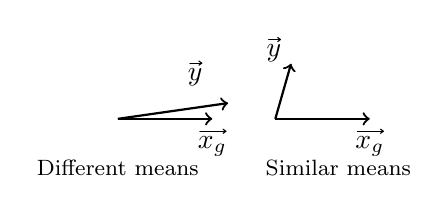
\begin{tikzpicture}[x=0.2cm, y=0.2cm]

% different means
\draw[thick,->] (-10,0) -- (-4,0);
\draw (-4,0) node[below] {$\vec{x_g}$};

\draw[thick,->] (-10,0) -- (-3,1);
\draw (-4,1.5) node[above left] {$\vec{y}$};
\draw (-10,-2) node[below,font=\footnotesize] {Different means};

% Similar means
\draw[thick,->] (0,0) -- (6,0);
\draw (6,0) node[below] {$\vec{x_g}$};

\draw[thick,->] (0,0) -- (1,3.5);
\draw (1,3) node[above left] {$\vec{y}$};
\draw (4,-2) node[below,font=\footnotesize] {Similar means};

\end{tikzpicture}

\end{center}

\end{frame}
%===========================================================



%===========================================================
\begin{frame}
  \frametitle{Multi-group One-way ANOVA as Regression}

\begin{itemize}

\item Exactly the same idea applies to $g$ groups, except now instead of one grouping variable, we define $g-1$ grouping variables, $\dim(X_g) = g-1$.

\item Then we calculate the multiple regression as we did before:

\end{itemize}

$$
\Mtx{y} = \Mtx{X}\Mtx{b} + \Mtx{e}
$$

$$
\Mtx{y} = \left[ \begin{array}{c}
y_1 \\ y_2 \\ \vdots \\y_n \\
\end{array}
\right]
\;
;
\;
\Mtx{X} = \left[ \begin{array}{ccccc}
1 & x_{11} & x_{12} & \cdots & x_{1g} \\
1 & x_{21} & x_{22} & \cdots & x_{2g} \\
\vdots & \vdots & \vdots & \vdots & \vdots \\
1 & x_{n1} & x_{n2} & \cdots & x_{ng} \\
\end{array}
\right]
\;
;
$$
%
Estimate \Mtx{b} as:
$$
\Mtx{b} = (\Mtx{X}^T \Mtx{X})^{-1}\Mtx{X}^T\Mtx{y}
$$

\end{frame}
%===========================================================

%===========================================================
\begin{frame}
  \frametitle{How Do We Construct the Grouping Matrix, $X_g$?}

Two common methods are:

\begin{enumerate}
\item Dummy coding -- define a set of $g$ grouping variables, where values take either 0 or 1, depending on group membership, but \emph{use only the first} $g-1$ columns:
%
\begin{equation*}
U_j = \left\{
\begin{aligned}
1, &\qquad \text{for every subject in group } j, \\
0, &\qquad \text{for all other subjects.}
\end{aligned}
\right.
\end{equation*}
and
%
$$
X_g= [U_1, U_2, \cdots, U_{g-1}]
$$
%
\item Effect (deviation) coding -- define the $U_j$ as above, and set:
$$
X_g = [U_1 - U_g, U_2-U_g, \cdots, U_{g-1} - U_g]
$$
\end{enumerate}


In general, effect coding is more similar to standard ANOVA contrasts. See this \href{http://www.ats.ucla.edu/stat/r/library/contrast_coding.htm}{\weblink\ web-page} for a more in depth discussion of different coding schemes. 

\end{frame}
%===========================================================


%===========================================================
\begin{frame}[fragile]
  \frametitle{ANOVA: Example Data Set}
\small
\begin{center}
\begin{tabular}{lrrrrr}
  \toprule
  & $g_1$ & $g_2$ & $g_3$ & $g_4$ \\
  \midrule
  & 20 & 21 & 17 & 8 & \\
  & 17 & 16 & 16 & 11 &  \\
  & 17 & 14 & 15 & 8 & \\
  \midrule
$M_{g.}$ & 18& 17 & 16 & 9 & $M_{..}=15$ \\
\bottomrule
\end{tabular}
\end{center}
%
\footnotesize
\begin{equation*}
y = \begin{bmatrix}
20 \\ 17 \\ 17 \\
21 \\ 16 \\ 14 \\
17 \\ 16 \\ 15 \\
8 \\ 11 \\ 8
\end{bmatrix}
,\qquad
\Mtx{X} = \begin{bmatrix}
1 & 1 & 0 & 0 \\
1 & 1 & 0 & 0 \\
1 & 1 & 0 & 0 \\
1 & 0 & 1 & 0 \\
1 & 0 & 1 & 0 \\
1 & 0 & 1 & 0 \\
1 & 0 & 0 & 1 \\
1 & 0 & 0 & 1 \\
1 & 0 & 0 & 1 \\
1 & -1 & -1 & -1 \\
1 & -1 & -1 & -1 \\
1 & -1 & -1 & -1
\end{bmatrix}
\end{equation*}
\end{frame}
%===========================================================

%===========================================================
\begin{frame}[fragile]
  \frametitle{ANOVA: Example Data Set, cont}
\small

Solving for $\Mtx{b}$ we find:

\begin{equation*}
\Mtx{b} = \begin{bmatrix}
15 \\ 3 \\ 2 \\ 1
\end{bmatrix},
\; \quad |\hat{\Mtx{y}}|^2 = 150, \;|\Mtx{e}|^2 = 40
\end{equation*}
Since, $\dim(\mathcal{V}_x) = 3$, and $\dim(\mathcal{V}_e)= 8$,  we get:
\begin{equation*}
  F = \frac{\dim(\mathcal{V}_e)|\vec{\hat{y}}|^2}
              {\dim(\mathcal{V}_x)|\vec{e}|^2}
    = 10
\end{equation*}

Here's the more conventional ANOVA table for the same data:
\footnotesize
\begin{center}
\begin{tabular}{lrrrrr}
  \toprule
 Source & df & $SS$ & $MS$ & $F$ & $\Pr(F)$ \\
  \midrule
 Experimental  & 3 & 150 & 50 & 10 & .0044\\
 Error  & 8  & 40 & 5 & \\
 \midrule
 Total & 11 & 190 & &\\
\bottomrule
\end{tabular}
\end{center}


\end{frame}
%===========================================================


%===========================================================
\begin{frame}[fragile]
  \frametitle{More Complex ANOVA models}

\begin{itemize}

\item Multi-way ANOVA -- used when samples are classified with respect to two or more factors (grouping variables). Allow for exploring interactions between facdtors.

\item Nested ANOVA -- used when there is more than one grouping variable, and the grouping variables form a nested hieararchy (groups, subgroups, subsubgroups)

\end{itemize}

As before, all of these can be treated as regression problems with appropriate design matrices!

\end{frame}
%===========================================================




%===========================================================
\begin{frame}
  \frametitle{Logistic Regression}
  
Logistic regression is used when the dependent variable is discrete (often binary).  The explanatory variables may be either continuous or discrete.
\medskip

Examples:
\begin{itemize}
\item whether a gene is turned off (=0) or on (=1) as a function of levels of various proteins
\item whether an individual is healthy (=0) or diseased (=1) as a function of various risk factors.
\end{itemize}

Model the binary responses as:

\[P(Y = 1|X_1,\ldots,X_p) = g^{-1}(\beta_1\Mtx{x}_1 + \beta_2\Mtx{x}_2 + \cdots + \beta_p\Mtx{x}_p)
\]

So we're modeling the probability of the states as a function of a linear combination of the predictor variables.

\end{frame}

%===========================================================
\begin{frame}
  \frametitle{Logistic Regression, Logit Transform}

Most common choice for $g$ is the `logit link' function:
\[
g(\pi) = log\left( \frac{\pi}{1-\pi} \right) 
\]

and $g^{-1}$ is thus the logistic function:

\[
g^{-1}(z) = \frac{e^z}{1+e^z}
\]

\end{frame}

%===========================================================
\begin{frame}
  \frametitle{Logistic Regression}

\[
P(Y = 1 | X) = \frac{e^{X\beta}}{1+e^{X\beta}}
\]

\bigskip

\begin{center}
\asyinclude[height=1.25in,keepAspect=true]{logistic-fxn.asy}
\end{center}

\end{frame}

%===========================================================
\begin{frame}
  \frametitle{Notes on Logistic Regression}

\begin{itemize}
    \item The regression is no longer linear
    \item Estimating the $\beta$ in logistic regression is done via maximum likelihood estimation (MLE)
    \item Information-theoretic metrics of model fit rather than F-statistics
\end{itemize}

\end{frame}

%===========================================================
\begin{frame}
  \frametitle{Logistic Regression Example}
  
\begin{figure}
\begin{center}
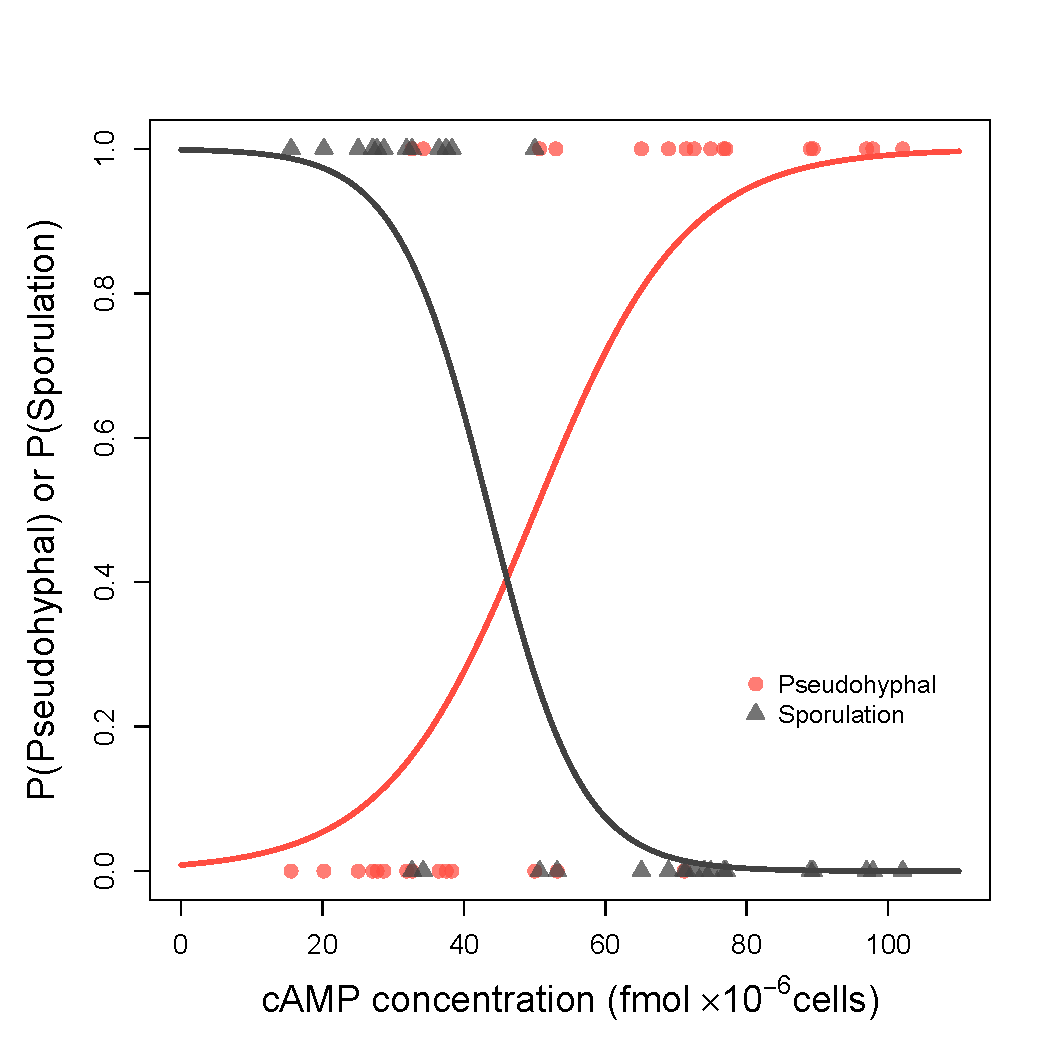
\includegraphics[height=2.5in]{cAMP-binary-model}
\end{center}
\caption{Logistic regression for yeast developmental phenotypes as a function of cAMP concentration.}
\end{figure}




\end{frame}
%===========================================================




%===========================================================
\begin{frame}
  \frametitle{Loess Regression}
  
\begin{itemize}
    \item A type of non-parametric regression
    \item Basic idea -- fit a curve (or surface) to a set of data by fitting a large number of \emph{local regressions}.
    \item Cleveland, W.S. (1979). ``Robust Locally Weighted Regression and Smoothing Scatterplots". Journal of the American Statistical Association 74 (368): 829-836. doi:10.2307/2286407.
\end{itemize}

\begin{center}
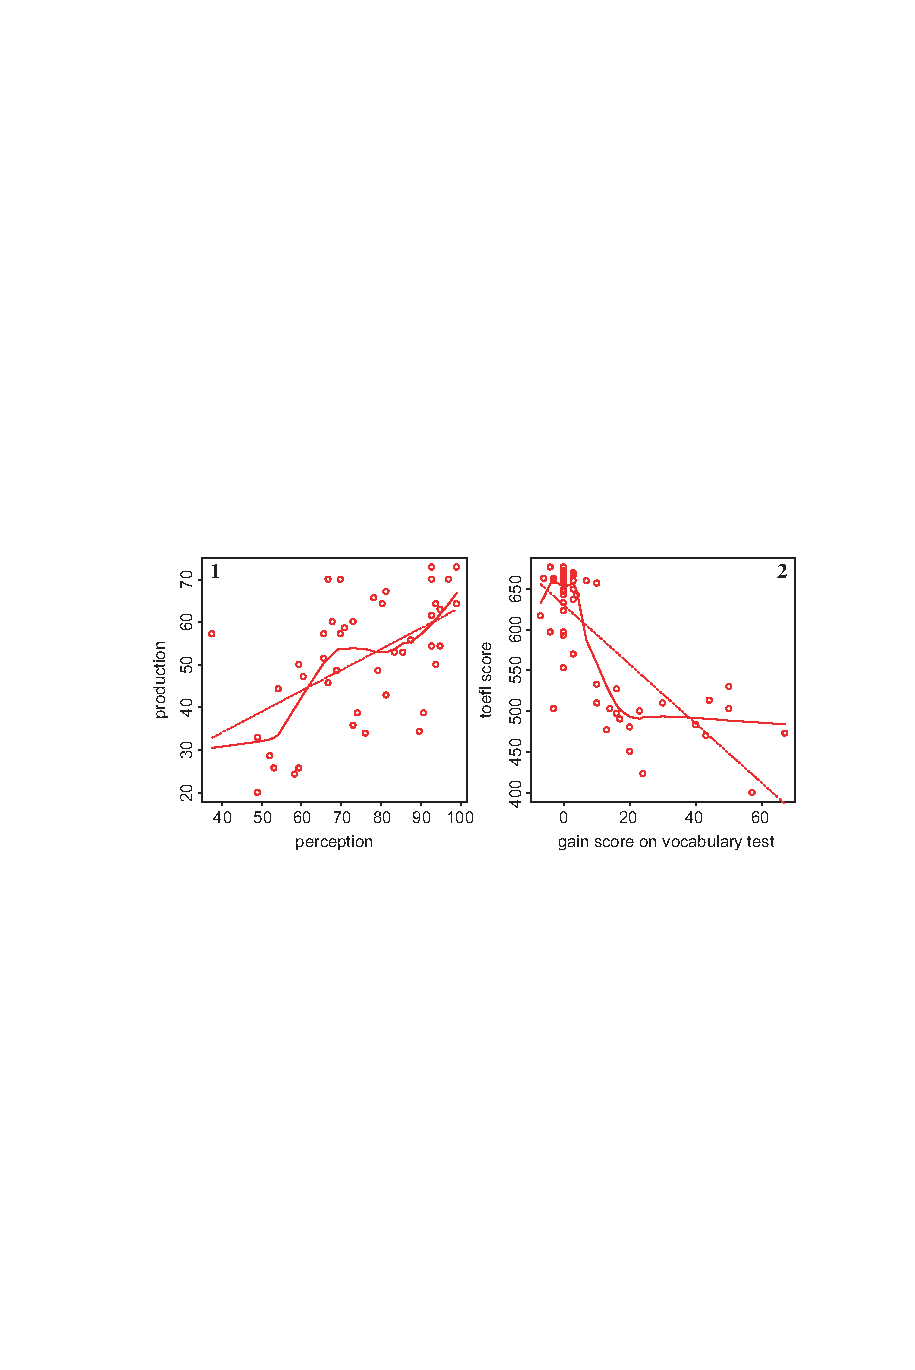
\includegraphics[height=1.25in]{loess-example.pdf}
\end{center}  


\end{frame}

%===========================================================
\begin{frame}
  \frametitle{Graphical overview of Loess fitting, I}  

{\tiny from Cleveland (1993)}
\begin{center}
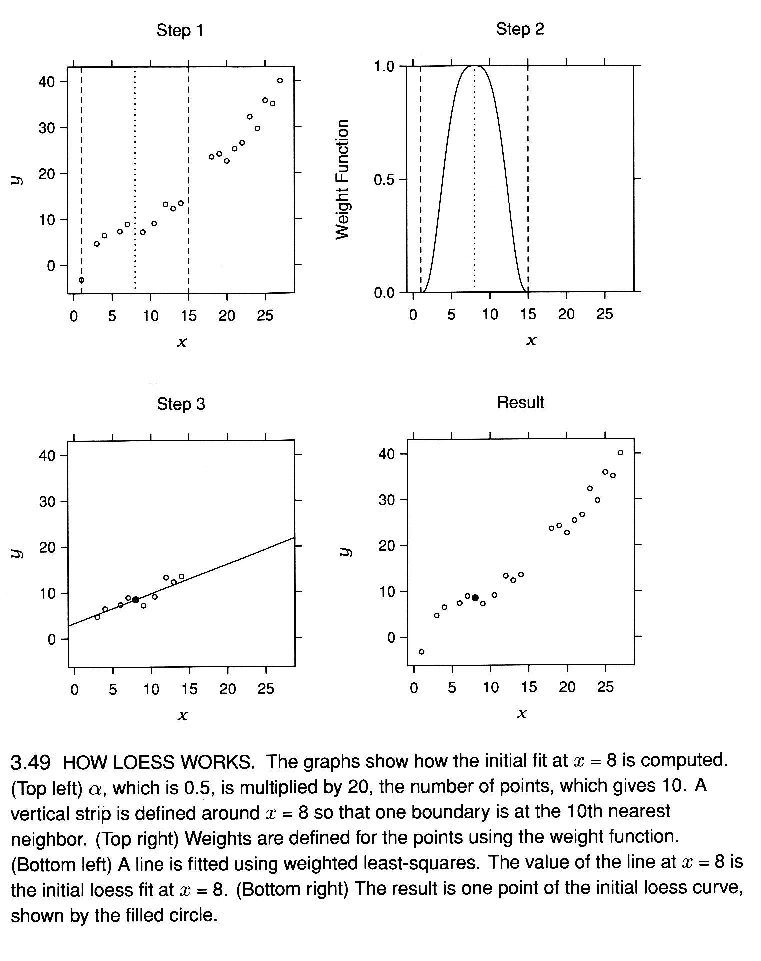
\includegraphics[height=3in]{loess1.pdf}
\end{center}  

\end{frame}

%===========================================================
\begin{frame}
  \frametitle{Graphical overview of Loess fitting, II}  

{\tiny from Cleveland (1993)}
\begin{center}
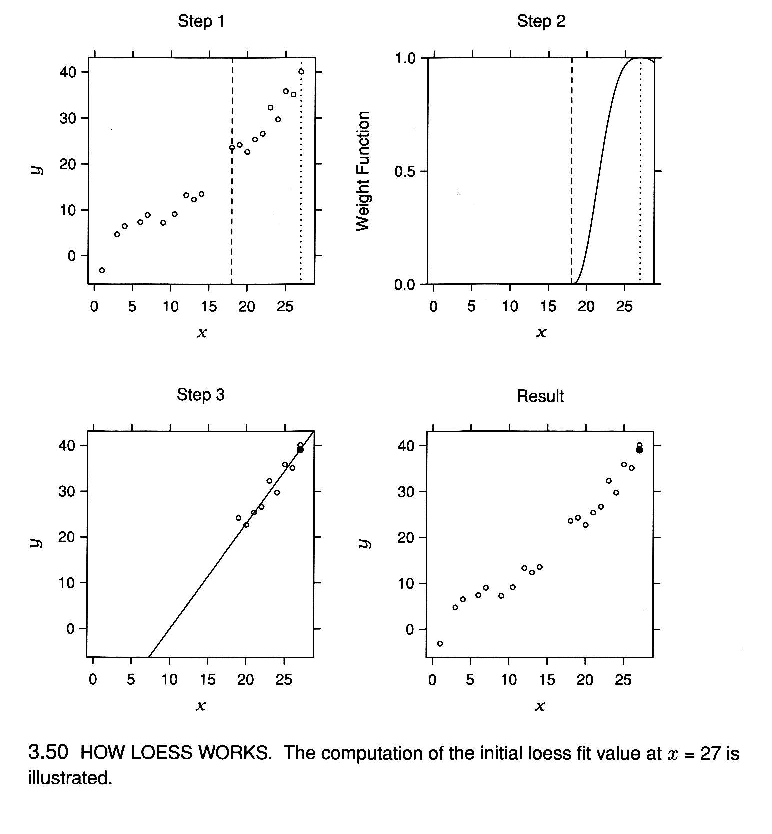
\includegraphics[height=3in]{loess2.pdf}
\end{center}  

\end{frame}

%===========================================================
\begin{frame}
  \frametitle{Graphical overview of Loess fitting, III}  

{\tiny from Cleveland (1993)}
\begin{center}
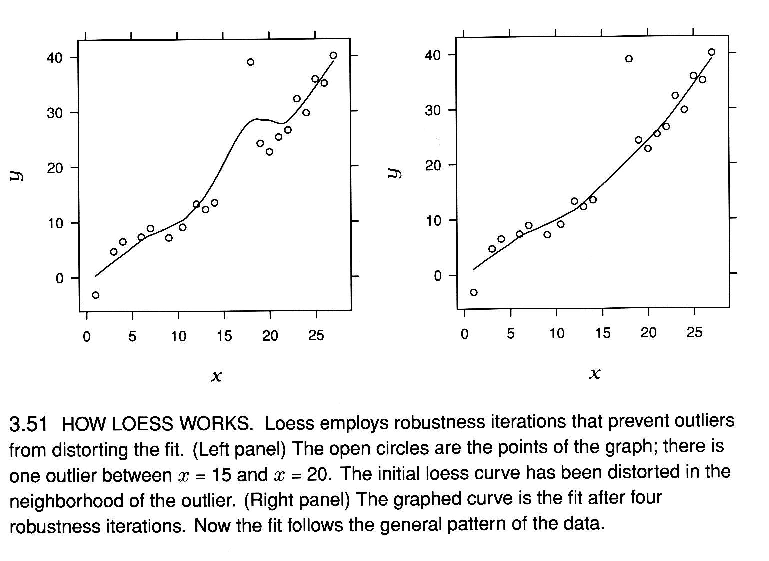
\includegraphics[height=3in]{loess3.pdf}
\end{center}  

\end{frame}



%===========================================================



\end{document}


%===========================================================
\begin{frame}
  \frametitle{XXX}

\end{frame}
%===========================================================
